
Aquí se realizará una exploración general de soluciones para indagar su
efectividad, esta exploración va guiada por el conocimiento del dominio y del
experto para asegurar su aplicabilidad final. No es necesario buscar en todo el
espectro de modelos, por ejemplo, el análisis de lenguaje natural se puede
resolver eficazmente con las Redes Neuronales,  gracias a esto el universo a
explorar será de arquitecturas. Esta fase puede ser muy intensiva
computacionalmente, así que la cantidad de iteraciones está limitada, como ya
sabemos el problema radica en que no existe una forma de determinar que modelo
será el mejor para un problema en particular.

En nuestro caso, ya hemos delimitado el tipo de algoritmo a utilizar. Si se
tiene \hyperlink{abbr}{BD} tabular, se procedería a: Probar modelos lineales,
bayesianos, Máquinas de Soporte Vectorial, Árboles Aleatorios, Redes Neuronales
y demás, usando parámetros estándar para estimar su rendimiento.

Para cada modelo, es preferible utilizar una validación cruzada y comparar tanto
la media como la desviación estándar. En algoritmos como las
\hyperlink{abbr}{ConvNet}s, esto puede ser difícil debido a la complejidad
computacional. También lo es determinar el tipo de error estadístico de cada
modelo para corroborar el impacto que tendrá tal error en el rendimiento del
algoritmo en situaciones de la vida real, por ejemplo, en el área médica es
importante la tasa de falsos positivos y falsos negativos.

Este proceso es naturalmente iterativo. Donde cambios en algoritmos,
arquitecturas e hiperparámetros obviamente modifican el rendimiento de los
algoritmos. El objetivo es encontrar un subconjunto muy reducido de candidatos a
probar, ya que estamos limitados por el tiempo y la complejidad computacional de
algunos modelos, que inclusive llegan a tardar semanas en entrenarse.

\subsection{Probar distintos algoritmos}

Se han probado varias arquitecturas desde las más grandes hasta las más
eficientes, todas ellas implementadas en lenguaje Python utilizando
\textbf{Keras}. El \emph{Zoológico de Modelos} es el término que engloba
arquitecturas de \hyperlink{abbr}{ConvNet}s pre-entrenadas para diversas tareas
de \hyperlink{abbr}{VC} (\emph{ImageNet}) y por lo general se manejan con
licencias libres, lo cual permite su implementación para resolver tanto
problemas generales como particulares si se aplica \hyperlink{abbr}{TL}.

La elección de estos algoritmos está basada directamente en la elección del
software utilizado para el desarrollo. Por lo que nos enfocaremos en el
\emph{Zoológico de Modelos} de \textbf{Keras} y su \emph{backend}:
\textbf{TensorFlow}. Para la búsqueda del mejor candidato a modelo solución se
realizó un experimento de búsqueda exhaustiva por todo el espacio de soluciones
comprendido dentro del \emph{Zoológico de Modelos} de \textbf{Keras}. Para ello
se programó un script automatizado que alimenta el ciclo de entrenamiento con
cada modelo de este espacio y captura los resultados del entrenamiento por
época, así como las métricas como la pérdida y la exactitud de cada iteración
del experimento.

\subsubsection{Arquitecturas probadas}

Las arquitecturas probadas fueron las siguientes y serán entrenadas con los
mismos hiperparámetros y el mismo número de épocas
(\autoref{fig:hiper_transfer}):

\begin{enumerate}
    \item DenseNet201
    \item InceptionResNetV2
    \item InceptionV3
    \item MobileNet
    \item MobileNetV2
    \item NASNetLarge
    \item NASNetMobile
    \item ResNet50
    \item VGG16
    \item VGG19
    \item Xception
\end{enumerate}

\begin{figure}[H]
    \centering
    \begin{minted}{python}
                            BATCH_SIZE = 64
                            FC_LAYERS = [1024, 1024]
                            LR = 0.00001
                            OPT = Adam(lr=LR)
                            EPOCHS = 20
                            DROPOUT = 0.5
    \end{minted}
    \caption{Hiperparámetros para búsqueda de algoritmos}\label{fig:hiper_transfer}
\end{figure}

\subsection{Comparar rendimiento}

Los resultados de los experimentos, sus gráficas, tablas y por arquitectura se
muestran en el \autoref{appendix:comparativa}. También incluye una breve
interpretación individual para cada arquitectura y el comportamiento de sus
métricas tanto en entrenamiento como en validación.

\subsection{Analizar métricas}

El análisis de las exactitudes de las arquitecturas probadas tanto en validación
como en entrenamiento se muestra en la~\autoref{fig:comp_total}. Podemos ver que
el comportamiento en entrenamiento fue bastante similar en todas las redes. Esto
cambió drásticamente en la fase de validación, donde la familia VGG se destacó
por sobre todas las demás. Así como en la exactitud, la pérdida se comportó
bastante similar en todos los modelos en la fase de entrenamiento. En
la~\autoref{fig:comp_totalloss} se muestra que algunas arquitecturas se
comportaban peor al pasar las épocas.

\begin{figure}[H]
    \centering
    \begin{subfigure}[b]{0.8\textwidth}
        \centering
       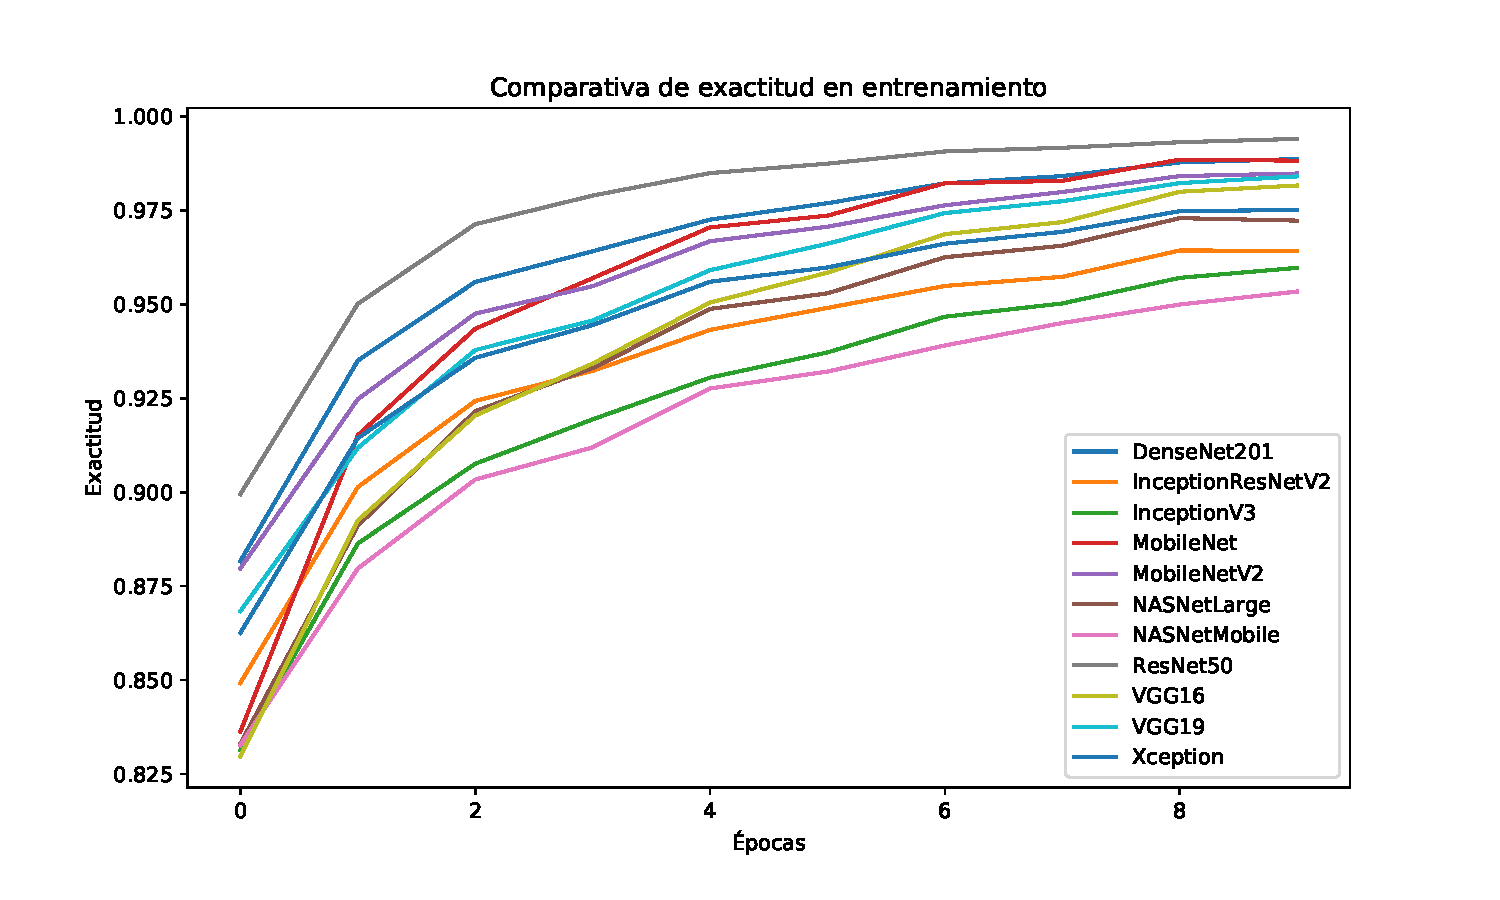
\includegraphics[width=1\textwidth]{capitulo_sdac/exactitud_entrenamiento.pdf}
       \caption{Exactitud en entrenamiento}\label{fig:comp_ent} 
    \end{subfigure}

    \begin{subfigure}[b]{0.8\textwidth}
        \centering
       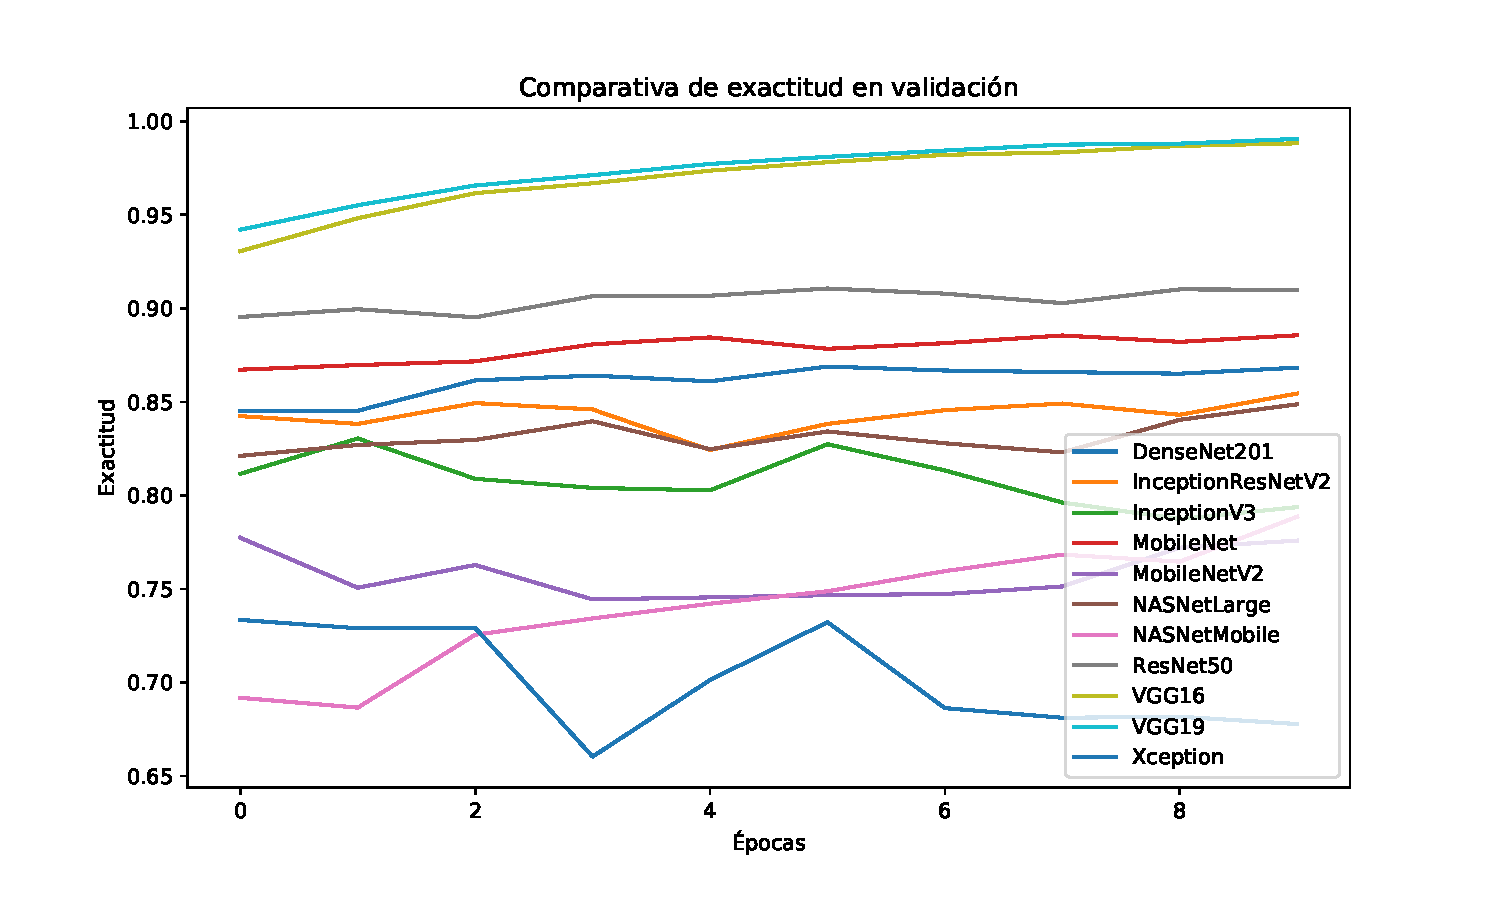
\includegraphics[width=1\textwidth]{capitulo_sdac/exactitud_validacion.pdf}
       \caption{Exactitud en validación}\label{fig:comp_val}
    \end{subfigure}
    \caption{Gráfica de comparativa de exactitud}\label{fig:comp_total}
\end{figure}
\begin{figure}[H]
    \centering
    \begin{subfigure}[b]{0.8\textwidth}
        \centering
       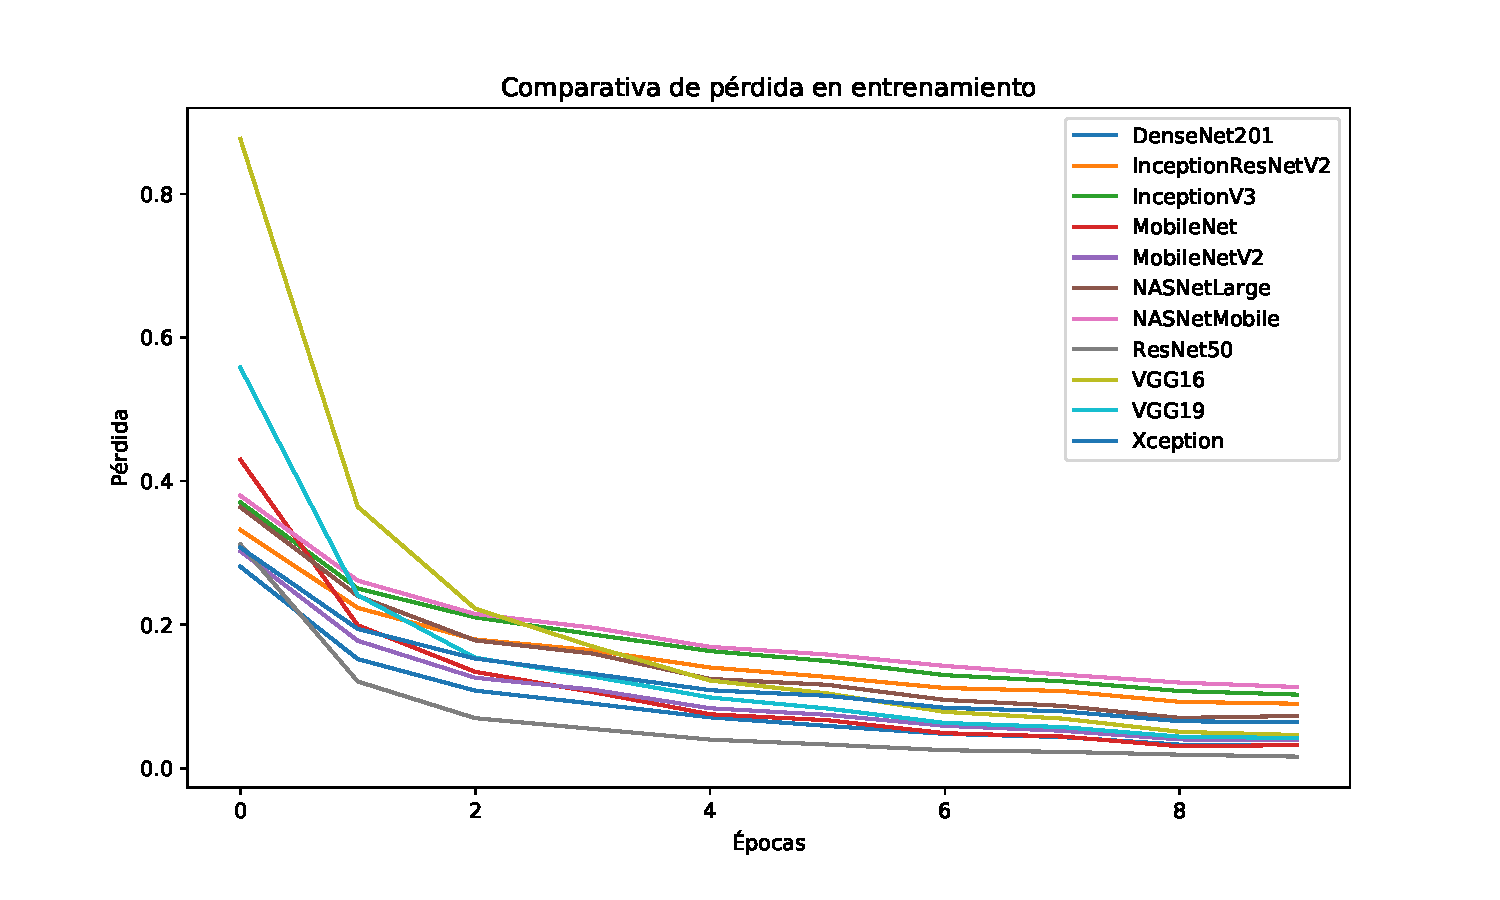
\includegraphics[width=1\textwidth]{capitulo_sdac/perdida_entrenamiento.pdf}
       \caption{Pérdida en entrenamiento}\label{fig:comp_entloss} 
    \end{subfigure}

    \begin{subfigure}[b]{0.8\textwidth}
        \centering
       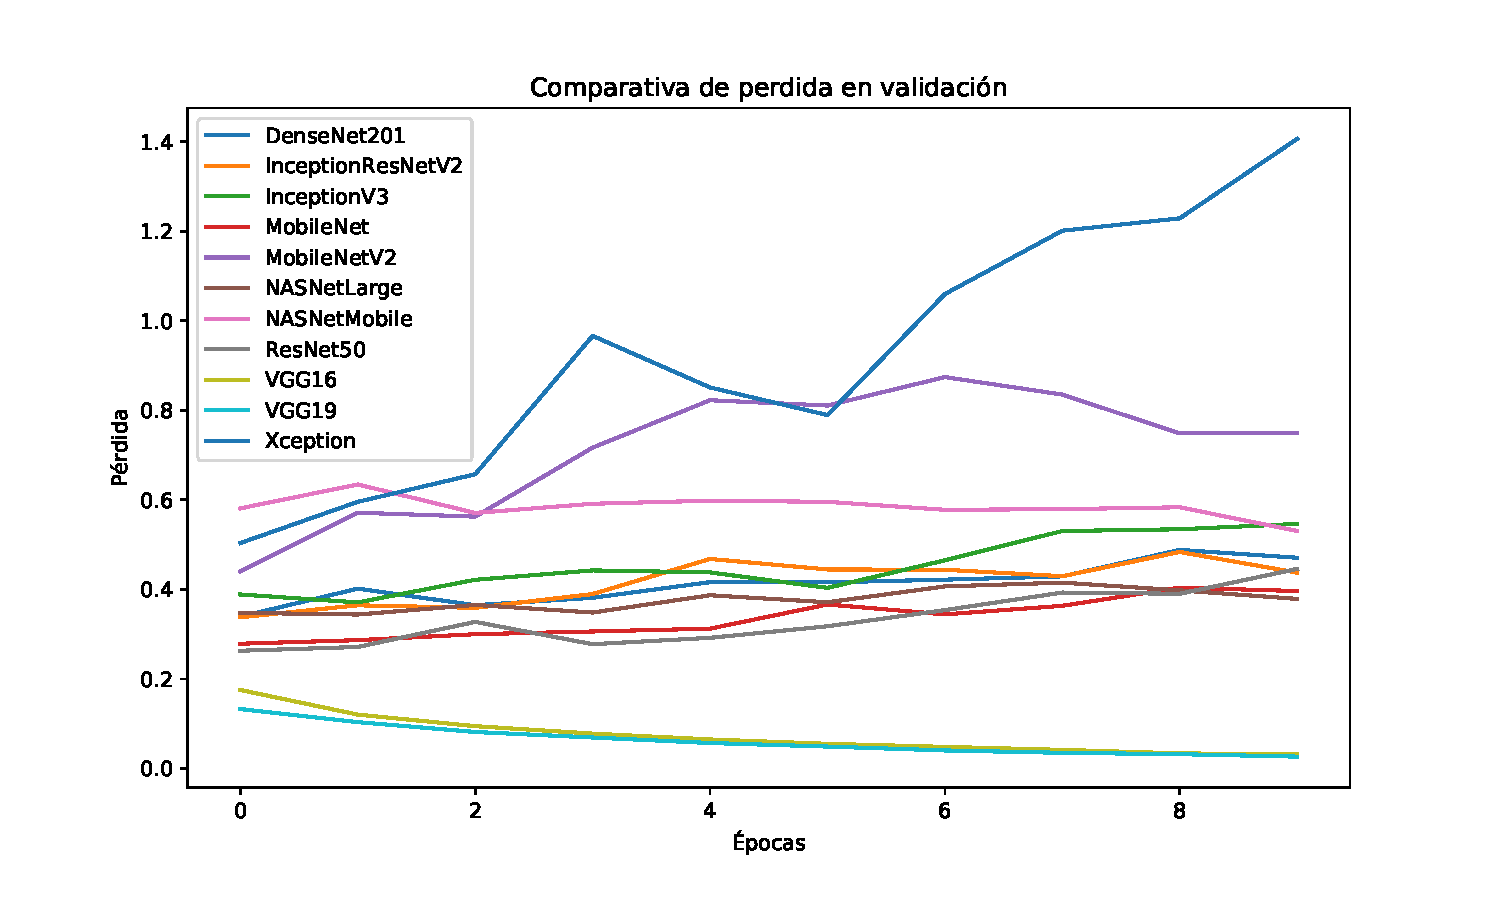
\includegraphics[width=1\textwidth]{capitulo_sdac/perdida_validacion.pdf}
       \caption{Pérdida en validación}\label{fig:comp_valloss}
    \end{subfigure}
    \caption{Gráfica de comparativa de pérdida}\label{fig:comp_totalloss}
\end{figure}

\subsection{Seleccionar los mejores algoritmos}

Una vez terminado el proceso de entrenamiento se requiere crear una lista con
los mejores modelos, teniendo siempre en mente la aplicabilidad final del
algoritmo. Pueden existir algoritmos con mejor rendimiento que por sus
características los hacen imposibles de implementar en el área donde surge el
problema. Por ejemplo, las \hyperlink{abbr}{RNA} son restrictivas en su
aplicación y prefieren ser desplegadas en sistemas donde se tenga disponible un
\hyperlink{abbr}{GPU} para realizar los cálculos.

\subsubsection{Algoritmo ganador}

Claramente los ganadores son las arquitecturas VGG16 y VGG19 entrenadas con
\emph{ImageNet}, alcanzando esta última una mejor exactitud en el mismo número
de épocas. Sabemos que esta arquitectura es suficientemente ligera para ser
implementada tanto en dispositivos móviles como en sistemas embebidos, en dado
caso que su tamaño impida una implementación con un rendimiento adecuado, se
puede optar por utilizar la VGG16 por su menor tamaño. Descubrir la razón por la
cual algunas arquitecturas se comportaban pésimo durante el experimento está
fuera del espectro de esta tesis, así como la búsqueda de otros modelos que
puedan resultar aptos y no estén implementados en \textbf{Keras} como las otras
arquitecturas de ResNet o CaffeNet.

Para segmentación semántica, solamente probaremos un algoritmo: Unet, ya que por
sus características, debido a las restricciones de tiempo y a su rendimiento
probado en aplicaciones citológicas, es claramente la mejor arquitectura para
este experimento. Esta arquitectura no implementará \hyperlink{abbr}{TL}. 

\subsection{Experimento}

Teniendo las arquitecturas o algoritmos ganadores, se puede diseñar un
experimento. El cual realizarse con todas las disposiciones
estadísticas para estimar correctamente el rendimiento del algoritmo en cada
iteración del proceso. El experimento consistirá en cambiar los hiperparámetros
del algoritmo para encontrar los mejores y asegurar un mejor rendimiento.
Existen distintas maneras de realizar este proceso pero están fuera del espectro
de esta tesis.

Al realizar el experimento, debemos de tener especial atención en guardar
absolutamente todos los cambios que se hagan tanto al algoritmo como a los
hiperparámetros, para poder analizar correctamente el rendimiento del modelo. El experimento
debe tener las siguientes características~\cite{Broman2017}:

\begin{enumerate}
    \item{\textbf{Repetible:}} Es la capacidad de volver a hacer el experimento
    en otro entorno ajeno al del investigador original y con un código
    independiente al entorno inicial de investigación.
    \item{\textbf{Reproducible:}} Un estudio es reproducible si se pueden tomar
    los datos originales y el código computacional usado para analizarlos y
    reproducir todos los hallazgos numéricos del estudio.
    \item{\textbf{Replicable:}} Es el acto de repetir un estudio completo,
    independientemente del investigador original sin el uso de datos originales
    y utilizando los mismos métodos.
\end{enumerate}